\documentclass{article}\usepackage[]{graphicx}\usepackage[]{color}
%% maxwidth is the original width if it is less than linewidth
%% otherwise use linewidth (to make sure the graphics do not exceed the margin)
\makeatletter
\def\maxwidth{ %
  \ifdim\Gin@nat@width>\linewidth
    \linewidth
  \else
    \Gin@nat@width
  \fi
}
\makeatother

\definecolor{fgcolor}{rgb}{0.345, 0.345, 0.345}
\newcommand{\hlnum}[1]{\textcolor[rgb]{0.686,0.059,0.569}{#1}}%
\newcommand{\hlstr}[1]{\textcolor[rgb]{0.192,0.494,0.8}{#1}}%
\newcommand{\hlcom}[1]{\textcolor[rgb]{0.678,0.584,0.686}{\textit{#1}}}%
\newcommand{\hlopt}[1]{\textcolor[rgb]{0,0,0}{#1}}%
\newcommand{\hlstd}[1]{\textcolor[rgb]{0.345,0.345,0.345}{#1}}%
\newcommand{\hlkwa}[1]{\textcolor[rgb]{0.161,0.373,0.58}{\textbf{#1}}}%
\newcommand{\hlkwb}[1]{\textcolor[rgb]{0.69,0.353,0.396}{#1}}%
\newcommand{\hlkwc}[1]{\textcolor[rgb]{0.333,0.667,0.333}{#1}}%
\newcommand{\hlkwd}[1]{\textcolor[rgb]{0.737,0.353,0.396}{\textbf{#1}}}%

\usepackage{framed}
\makeatletter
\newenvironment{kframe}{%
 \def\at@end@of@kframe{}%
 \ifinner\ifhmode%
  \def\at@end@of@kframe{\end{minipage}}%
  \begin{minipage}{\columnwidth}%
 \fi\fi%
 \def\FrameCommand##1{\hskip\@totalleftmargin \hskip-\fboxsep
 \colorbox{shadecolor}{##1}\hskip-\fboxsep
     % There is no \\@totalrightmargin, so:
     \hskip-\linewidth \hskip-\@totalleftmargin \hskip\columnwidth}%
 \MakeFramed {\advance\hsize-\width
   \@totalleftmargin\z@ \linewidth\hsize
   \@setminipage}}%
 {\par\unskip\endMakeFramed%
 \at@end@of@kframe}
\makeatother

\definecolor{shadecolor}{rgb}{.97, .97, .97}
\definecolor{messagecolor}{rgb}{0, 0, 0}
\definecolor{warningcolor}{rgb}{1, 0, 1}
\definecolor{errorcolor}{rgb}{1, 0, 0}
\newenvironment{knitrout}{}{} % an empty environment to be redefined in TeX

\usepackage{alltt}
\usepackage{amscd, amssymb, amsmath, verbatim, setspace}
\usepackage[left=1.0in, right=1.0in, top=1.0in, bottom=1.0in]{geometry}
\usepackage{mathrsfs}
\usepackage{listings}


\IfFileExists{upquote.sty}{\usepackage{upquote}}{}
\begin{document}

\begin{flushright}
  Arif Ali\\
  ANLY-511 Prob. Modeling \& Stat. Computing\\
	Oct 29, 2015\\
\end{flushright}

\begin{center}
  \LARGE\textbf{Homework \#7}
\end{center}
\section*{Problem 49}
\begin{knitrout}
\definecolor{shadecolor}{rgb}{1, 1, 1}\color{fgcolor}\begin{kframe}
\begin{verbatim}
data("chickwts")
boxplot(weight~feed, data = chickwts)
\end{verbatim}
\end{kframe}
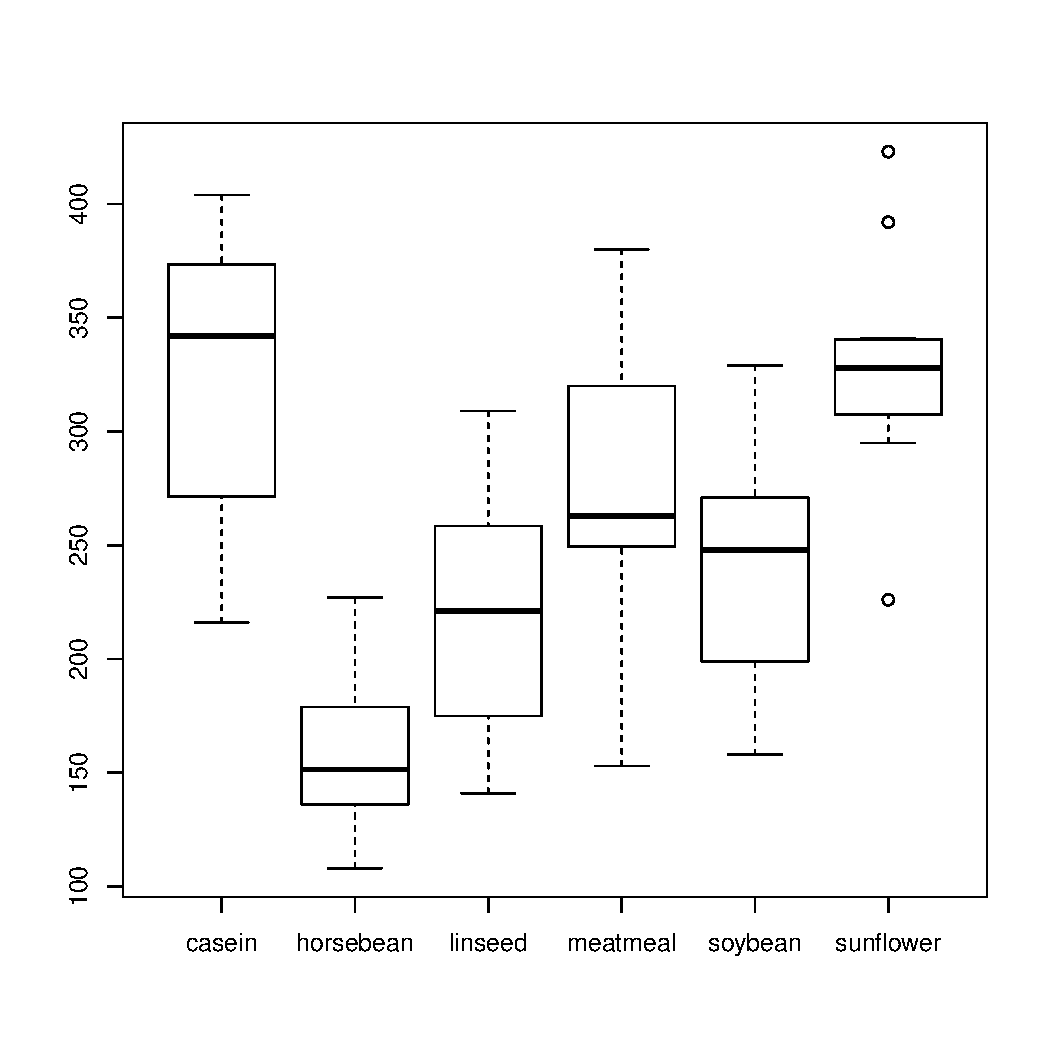
\includegraphics[width=0.33\linewidth]{figure/unnamed-chunk-2-1} 

\end{knitrout}
The feed type with the biggest gain seems to be the Casein while horsebean seems to have the smallest gain in weight. The Casein has a much larger range, but it looks like the it has the highest median. Linseed and soybean seem to have around the saame weight gain. While soybean as slightly higher weight gain, the quantiles seem very close.
\section*{Problem 50}
\subsection*{Part A}
\begin{knitrout}
\definecolor{shadecolor}{rgb}{1, 1, 1}\color{fgcolor}\begin{kframe}
\begin{verbatim}
setwd("~/Dropbox/School/Georgetown/Analytics 511 Fall 2015/ChiharaHesterberg/")
GSS2006 = read.csv("GSS2006.csv")
table(GSS2006$DeathPenalty, GSS2006$Region)
##         
##          Mid-Atl Mountain New Engl North Central Pacific South Atlantic
##   Favor      203      176       59           429     279            431
##   Oppose     131       55       42           228     131            194
##         
##          South Central
##   Favor            308
##   Oppose           149
\end{verbatim}
\end{kframe}
\end{knitrout}
The death penalty is strongely favored in South Atlantic and South Central regions. Pacific and New England has significiantly less support for the death penalty. Overall, it looks like most people support the death penalty by a 2:1 ratio. There are so many things I could say regarding cultural differences that might lead to this.   
\subsection*{Part B}
\begin{knitrout}
\definecolor{shadecolor}{rgb}{1, 1, 1}\color{fgcolor}\begin{kframe}
\begin{verbatim}
table(GSS2006$Marijuana, GSS2006$Region)
##            
##             Mid-Atl Mountain New Engl North Central Pacific South Atlantic
##   Legal          80       61       37           165     113            133
##   Not legal     147       87       31           270     143            266
##            
##             South Central
##   Legal                83
##   Not legal           212
\end{verbatim}
\end{kframe}
\end{knitrout}
Mountain, New England, and the Pacific seem to have the strongest amount of support for legalizing. South Central and South Atlantic seem not as much in favor. Nationally, it's not a clearly Not legal as with the death penalty.
\subsection*{Part C}
\begin{knitrout}
\definecolor{shadecolor}{rgb}{1, 1, 1}\color{fgcolor}\begin{kframe}
\begin{verbatim}
table(GSS2006$Marijuana, GSS2006$DeathPenalty)
##            
##             Favor Oppose
##   Legal       408    229
##   Not legal   734    367
\end{verbatim}
\end{kframe}
\end{knitrout}

Areas that favor legalization seem to not as strongly favor the death penalty mainly New England, and the Pacific. The Mid-Atlantic and South Atlantic seems to be holding the same ratio in both situations. South Cental has a differing ratio but opposing the death penalty and legalizing as the losing choices. 
\section*{Problem 51}
\begin{knitrout}
\definecolor{shadecolor}{rgb}{1, 1, 1}\color{fgcolor}\begin{kframe}
\begin{verbatim}
x0 = function(n){
  return(qnorm(.95, 0, 1/sqrt(n)))
}
x0(20)
## [1] 0.3678005
\end{verbatim}
\end{kframe}
\end{knitrout}
\section*{Problem 52}
\begin{knitrout}
\definecolor{shadecolor}{rgb}{1, 1, 1}\color{fgcolor}\begin{kframe}
\begin{verbatim}
p0 = function(x0, n){
  return(pnorm(x0, 0, 1/sqrt(n), lower.tail = F))
}
p0(.4, 20)
## [1] 0.03681914
\end{verbatim}
\end{kframe}
\end{knitrout}

\section*{Problem 53}
\begin{knitrout}
\definecolor{shadecolor}{rgb}{1, 1, 1}\color{fgcolor}\begin{kframe}
\begin{verbatim}
power_test = function(ua, n, x0){
  pnorm(x0, ua, 1/sqrt(n), lower.tail = F)
}
power_test(.2,20,.5)
## [1] 0.08985625
power_test(1,20,.5)
## [1] 0.9873263
\end{verbatim}
\end{kframe}
\end{knitrout}

\section*{Problem 54}
\subsection*{Part A}
The distribution of $\bar(x)$ is $N(1, (\sqrt(\frac{8}{15}))^2)$
\subsection*{Part B}
\begin{knitrout}
\definecolor{shadecolor}{rgb}{1, 1, 1}\color{fgcolor}\begin{kframe}
\begin{verbatim}
pnorm(0.3, 1, sqrt(8/15), lower.tail = F)
## [1] 0.8310983
pnorm(1.1, 1, sqrt(8/15), lower.tail = F)
## [1] 0.4455428
pnorm(2.1, 1, sqrt(8/15), lower.tail = F)
## [1] 0.06600317
\end{verbatim}
\end{kframe}
\end{knitrout}
\subsection*{Part C}
\begin{knitrout}
\definecolor{shadecolor}{rgb}{1, 1, 1}\color{fgcolor}\begin{kframe}
\begin{verbatim}
xbar = replicate(10000, pnorm(mean(rnorm(15, 1, sqrt(8))),1 , sqrt(8/15), lower.tail = F))
hist(xbar)
\end{verbatim}
\end{kframe}
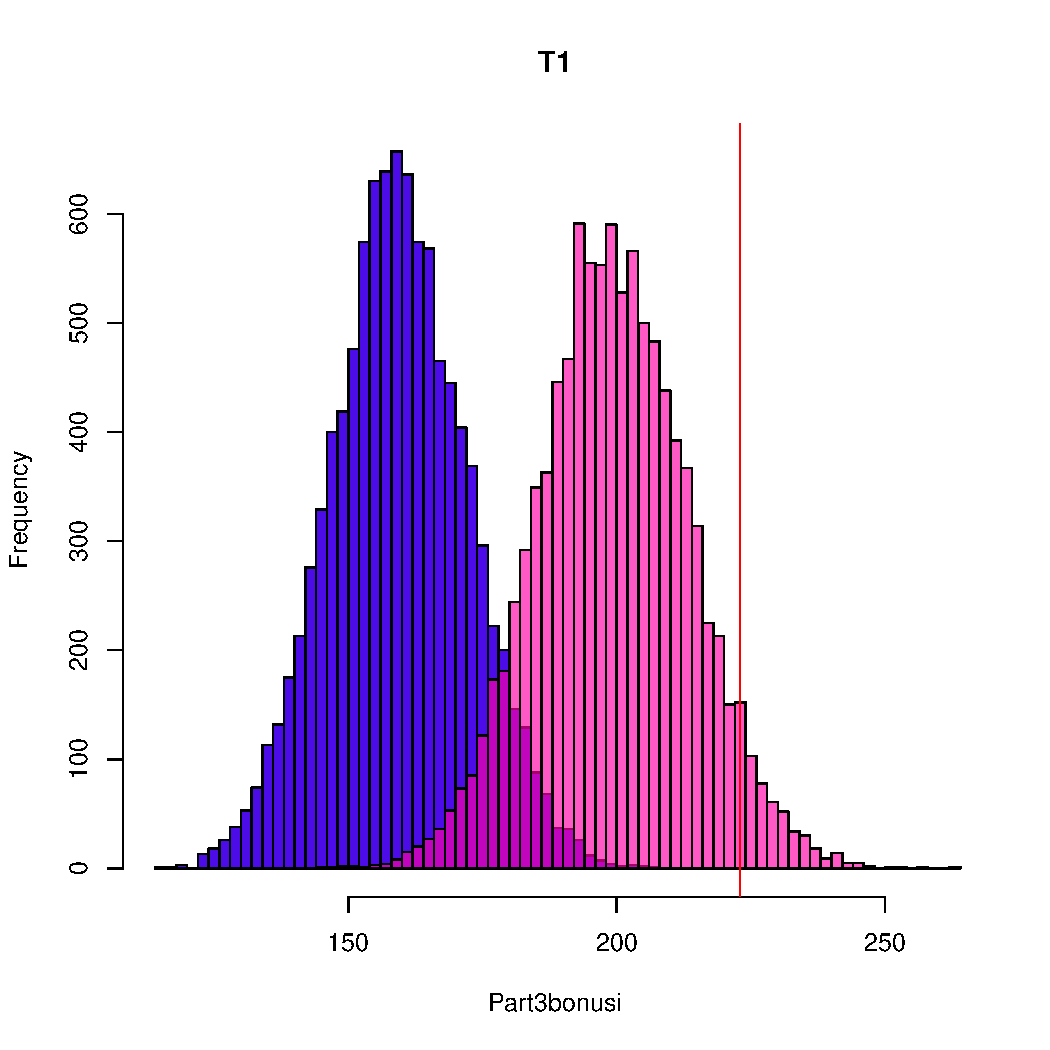
\includegraphics[width=0.33\linewidth]{figure/unnamed-chunk-10-1} 
\begin{kframe}\begin{verbatim}
plot.ecdf(xbar)
\end{verbatim}
\end{kframe}
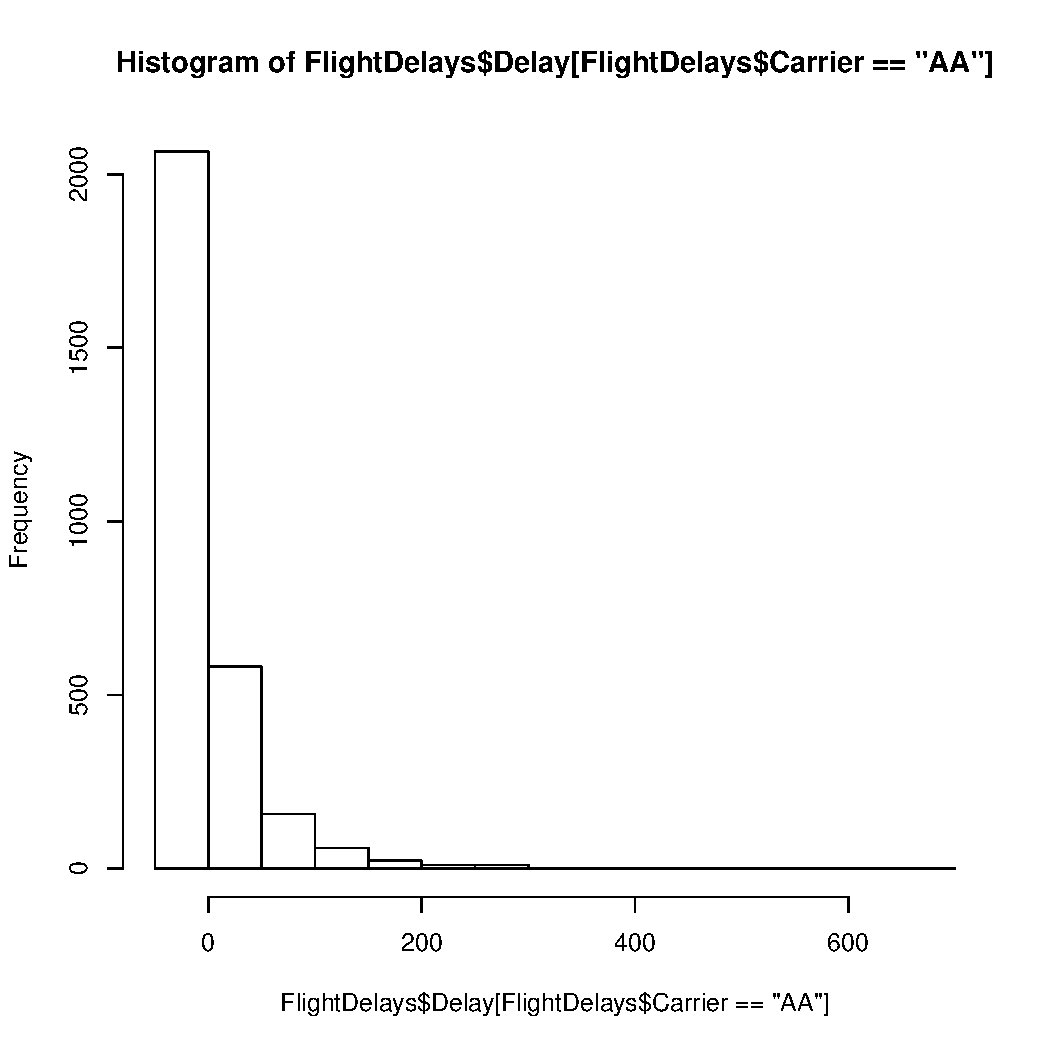
\includegraphics[width=0.33\linewidth]{figure/unnamed-chunk-10-2} 
\begin{kframe}\begin{verbatim}
# From both the ecdf and the histogram, the distribution of xbar under the null  
# hypothesis is uniform from a source. The idea that I have behind why the p values 
# is a uniform distribution is to be able to equally value each point's rejection area.  
# https://shihho.wordpress.com/2012/11/27/pvalue_distribution/, 
# the following is a proof from this wordpress of why that is possible.
\end{verbatim}
\end{kframe}
\end{knitrout}
Let $z=F(t)$

$P(X\geq t)=P(F(X)\geq F(t))=P(F(X)\geq z)$
$\implies 1-P(F(X)<z)=1-z$

$\therefore 1-P(F(X)<z)=1-z$

$z\in [0,1]$

$z = \int^{z}_{0} f(z') dz'\implies f(z)=1$ So z is uniform.

\section*{Problem 55}

The first part is not the permutation test, I wanted to calculate the actual p-value, so the following is the Chi-Square with 38 degrees of freedom.
\begin{knitrout}
\definecolor{shadecolor}{rgb}{1, 1, 1}\color{fgcolor}\begin{kframe}
\begin{verbatim}
setwd("~/Dropbox/School/Georgetown/Analytics 511 Fall 2015/ChiharaHesterberg/")
lottery = read.csv("Lottery.csv")
C = sum((table(lottery$Win)-500/39)^2/(500/39))
pchisq(C, 38, lower.tail = F)
## [1] 0.669616
\end{verbatim}
\end{kframe}
\end{knitrout}
Since $0.669616 > 0.05$, the null hypothesis continues to holds.

This is the permutation test. 
\begin{knitrout}
\definecolor{shadecolor}{rgb}{1, 1, 1}\color{fgcolor}\begin{kframe}
\begin{verbatim}
setwd("~/Dropbox/School/Georgetown/Analytics 511 Fall 2015/ChiharaHesterberg/")
lottery = read.csv("Lottery.csv")
lottonumbers = table(lottery)
expected <- mean(lottonumbers)

lottoX2 = function(x){return(sum((x - expected)^2/expected))}
lottoX2(lottonumbers)
## [1] 33.676
X2 = sum((lottonumbers - expected)^2/expected)

sim <- replicate(10000, lottoX2(rmultinom(1,500,rep(1/39,39))))

mean(sim > X2)
## [1] 0.6625
\end{verbatim}
\end{kframe}
\end{knitrout}
Once again, the $p-value > 0.05$, the null hypothesis probably holds.
\section*{Problem 56}
\begin{knitrout}
\definecolor{shadecolor}{rgb}{1, 1, 1}\color{fgcolor}\begin{kframe}
\begin{verbatim}
setwd("~/Dropbox/School/Georgetown/Analytics 511 Fall 2015/ChiharaHesterberg/")
titanic = read.csv("Titanic.csv")
observed = (mean(titanic$Age[titanic$Survived==1]) - mean(titanic$Age[titanic$Survived==0]))

N = 10^4-1 #Value from book
result = numeric(N)
for(i in 1:N){
  Survival.permuted = sample(titanic$Age, replace = F)
  result[i] = (mean(Survival.permuted[titanic$Survived==1]) 
               - mean(Survival.permuted[titanic$Survived==0]))
}
(sum(result < observed)+1)/(N+1)*2
## [1] 8e-04
\end{verbatim}
\end{kframe}
\end{knitrout}
The p-value is significiantly less than 0.05; therefore the null hypothesis is significiantly less likely to hold; therefore, we reject it. The p-value must by multipled by two since this is a two sided test.
\end{document}
